%\documentclass{sig-alternate}
\documentclass{sig-alternate-05-2015} % For MSR



  \pdfpagewidth=8.5truein
  \pdfpageheight=11truein



%% --- Author Metadata here ---
%\conferenceinfo{ISSTA'16,}{July 17-20, 2016, Saarbr�cken, Germany.}
%\CopyrightYear{2016} % Allows default copyright year (2002) to be over-ridden - IF NEED BE.
%\crdata{978-1-4503-3739-7/16/04...\$15.00.\\
%http://dx.doi.org/xx.xxxx/xxxxxxx.xxxxxxx
%}  % Allows default copyright data (X-XXXXX-XX-X/XX/XX) to be over-ridden.
%% --- End of Author Metadata ---


\usepackage{cite}
\usepackage{color}
\usepackage{balance}
\usepackage{times}
\usepackage{url}
\urlstyle{same} % formats footnotes
\usepackage{xcolor}
\usepackage{pgfplots}
\usepackage{soul} % highlighting
\usepackage{multirow}
\usetikzlibrary{patterns} %% Used for bar charts

\newcommand{\todo}[1]{\textcolor{cyan}{\textbf{[#1]}}}
\newcommand{\dan}[1]{\textcolor{blue}{{\it [Dan says: #1]}}}
\newcommand{\andy}[1]{\textcolor{blue}{{\it [Andy says: #1]}}}
\newcommand{\sam}[1]{\textcolor{blue}{{\it [Sam says: #1]}}}

% Define flow chart styles
\tikzstyle{decision} = [diamond, draw, fill=blue!20,
    text width=15em, text badly centered, node distance=3cm, inner sep=0pt]
\tikzstyle{block} = [rectangle, draw, fill=blue!20,
    text width=15em, text centered, rounded corners, minimum height=4em]
\tikzstyle{line} = [draw, -latex']

\usetikzlibrary{shapes,arrows, positioning} % Needed for analysis diagram


\newif\ifisnopii
\isnopiitrue % change to true/false to remove personally identifiable information (pii)
%\isnopiifalse % change to true/false to remove personally identifiable information (pii)


\begin{document}

%Mistakes and Malware: An Large Scale Analysis of Malicious and Google Play Android Apps
% Rotten Fruit and : An Large Scale Analysis of Malicious and Google Play Android Apps
%Quality and Security: A Large Scale Analysis of Malicious and Google Play Android Apps

%Quality and Security: An Analysis of 70,000 Google Play and Malicious Android Apps

\title{Mistakes and Malware: A Large Scale Analysis of Benign and Malicious Android Apps}


\numberofauthors{1}
\ifisnopii % turn on/off pii
\author{
%
% 1st. author\
\alignauthor
Daniel E. Krutz, Andrew Meneely, and Samuel A. Malachowsky\\ 	
	\affaddr{Software Engineering Department}\\
       \affaddr{Rochester Institute of Technology}\\
       \affaddr{1 Lomb Memorial Drive}\\
       \affaddr{Rochester, NY, USA} \\
       \email{\{dxkvse, axmvse, samvse\}@rit.edu}
       \alignauthor
} % Must not be a space above this

\else % turn on/off pii
\author{
%
% 1st. author
\alignauthor
xxxxxxxxxxxxxxx\\ 	
	\affaddr{xxxxxxxxx}\\
       \affaddr{xxxxxxxxx}\\
       \affaddr{xxxxxxxxx}\\
       \affaddr{xxxxxxxxx, xx, xxx} \\
       \email{xxxxxx@xxxxx.xxx}
       \alignauthor
} % Must not be a space above this
\fi % end turn on/off pii

\maketitle
\begin{abstract}

% 31,234
% 70,785
% 1,420 - malware


Android has become the world's most popular mobile platform, allowing users to perform a variety of tasks that were previously unachievable in a mobile environment. Unfortunately, Android applications (apps) are not immune to the problems which also plague conventional software including security vulnerabilities, quality defects, permission misuse, and numerous other issues. Many developers even intentionally create vulnerable or malicious apps (malware) for often highly lucrative purposes.

In order to create better software along with protect against malware, we need to better understand the current trends in the development and attributes of each of these groups. We collected and reverse engineered 70,785 Android apps from the Google Play store, along with 1,420 malicious apps from several other sources. The creation date of these apps ranged from early 2010 to late 2015. Each app was analyzed using several static analysis tools to record a variety of information about each of them including requested permissions, size (LOC), possible defects and permission misuse.

Our findings conclude that malware typically requests more permissions and suffers in several quality related metrics in comparison to benign apps, that malware and benign apps are annually growing both in terms of LOC and requested permissions, and  that apps in the `Communication'  category suffer from the highest rate of over-permissions while also requesting the most permissions. We also present an easy to use, robust website and dataset for others to use in their own research.


%\todo{Check on the overall malware number - this is different compared with my other findings}
%%% Provide another example of the dataset. Writing your own queries?


%% What other RQs could I add in to add some value to the paper?


% Is there a correlation between quality and security?
%	People are going to say that it was done before and how can you reverse engineer apps like that
% 




\end{abstract}

%% Categories taken from: http://www.jucs.org/ujs/jucs/links/Articles%20by%20Category/D.?mode=bc

%% >>> Add this as well? D.4.6 [Operating Systems]: Security and Protection

%\category{D.4.6}{Operating Systems}Security and Protection;
%\category{D.2.0}{Software Engineering} General;
%\category{D.2.0}{Software Engineering} General;

%% From the Code Clone paper
%\category{K.3.2}{Computers and Education}Computers and Information
%Science Education- Computer science education; Curriculum

\keywords{Android, Malware, Static Analysis}


\section{Introduction}

Android is the world's most popular mobile operating system and is expected to dominate the smartphone market until at least 2019~\cite{Risley_url}. Mobile applications (apps) are the programs that run on mobile devices and allow the user to do everything from post a Twitter message, to conduct banking transactions. In order to create better software, we need to better understand the current trends in development, and what are some of the most profound issues from a security perspective are. Some of areas which should be examined include permissions misuse, security vulnerabilities, defects, adherence to coding standards, and a variety of other metrics. 

%% Removed since I felt it was redundant
%Understanding current apps is important for learning how to create future apps cheaper, better, faster, and more secure. Android apps may be analyzed using static analysis tools which report on a variety of attributes including possible security vulnerabilities, adherence to coding standards, potential defects and size. Understanding existing apps may not only provide valuable information about current apps, but also in how to better create future apps as well.

Unfortunately, many apps are created with a sinister intent. Malware is striving to attack phones in a multitude of ways and is a highly lucrative business, generating revenue in several ways including sale of personal user information, stolen credentials, and premium-rate calls and SMS messages~\cite{felt2011survey}. Malware is a constant concern as recent studies have shown that nearly 20\% of Android apps are malware~\cite{tynan_dan_report:_2015}. To make matters worse, detecting malware is not easy. Even with a myriad of sophisticated detection systems, malware is often released to Google Play and is able to circumvent Bouncer, Google's malware protection mechanism for their store~\cite{bouncer_url1}. Many detection techniques are built on manually created detection patterns which do not always work well for discovering new malware instances~\cite{Zhou:2012:DAM:2310656.2310710}. In order to better detect and defend against malware, we need to understand more about it. Knowing how it is created, evolves, and its characteristics are all valuable pieces of information in the battle against malware.

In recent academic studies, static analysis tools have also been used as one method of measuring the quality and security of mobile software~\cite{Felt:2011:APD:2046707.2046779,Vidas11curbingandroid,Lee_2013}.  \emph{An empirical analysis of a large body of malicious and benign Android applications over time can therefore provide insights into these apps, and their trends.} % really work on making this good


% \emph{An empirical analysis of a large body of malicious and benign Android applications over time can therefore provide a broad view into how individual apps and app genres relate to one another and provide more insight on these apps.}


The goal of this work is to better understand benign and malicious apps Android apps through the use of static analysis. We collected and reverse engineered 70,785  Android applications in 41 different genres from the Google Play store along with 1,420 malware samples from Contagio Mobile Mini Dump~\cite{contagio_url} and the Malware Genome Project~\cite{Zhou:2012:DAM:2310656.2310710}. Each of the apps were analyzed using five static analysis tools: Stowaway~\cite{Felt:2011:APD:2046707.2046779}, Androrisk\footnote{\url{https://github.com/androguard/androguard}}, CheckStyle\footnote{\url{http://checkstyle.sourceforge.net/}}, Jlint\footnote{\url{http://jlint.sourceforge.net/}}, and APKParser\footnote{\url{https://github.com/joakime/android-apk-parser}}. We examined application size, rate of potential defects, adherence to coding standards, rate of over-permissions, and potential vulnerability level. An additional benefit of our work is a publicly available dataset and robust website which may be used by researchers, developers, students, and general Android users to better understand these apps.

Our research is guided by the following questions:\todo{update all of these \& add findings}

\textbf{RQ1:}~\emph{How do app genres compare in terms of quality metrics?}\\
We found that `Tools' apps suffer from the highest rate of coding standards defects per line of code (LOC), while `Communication' apps have the highest rate of over-permission.

........


%We compared the static analysis results for apps with less than 10,000 downloads against apps with more than 10,000 downloads to understand if there was a difference between more popular apps compared with ones which were more seldom used. We found that apps with at least 10,000 downloads averaged more LOC, while having fewer coding standards mistakes per LOC than apps with less than 10,000 downloads. We also found that apps with at least 10,000 downloads had a higher rate of potential defects per LOC according to Jlint.


%The rest of the paper is organized as follows: Section~\ref{sec: aboutcourse} describes the course including learning objectives. Section~\ref{sec: activity}\todo{finish}

The rest of the paper is organized as follows: Section~\ref{sec: relatedwork} discusses related works, while section~\ref{sec: androidapplications} describes the structure of Android apps. Section~\ref{sec: csa} provides details of how we collected the apps and conducted our static analysis on them. Section~\ref{sec: evaluation} discusses the results of our research questions and provides an analysis of our findings. Section~\ref{sec:dataset} presents information regarding our public dataset. Section~\ref{sec:limitations} discusses limitations of our research and future work to be conducted. Section~\ref{sec: conclusion} concludes our study.\dan{update all of this}
%\dan{make sure this is up to date}

\section{Related Work}
\label{sec: relatedwork}


There have been many studies which analyzed mobile apps on a large scale. Sarma~\emph{et al.} evaluated several large data sets, including one with 158,062 Android apps in order to gauge the risk of installing the app, with some of the results broken down by genre. However, this work did not analyze the apps using the range of static analysis tools which we used. Viennot~\emph{et al.} developed a tool called `PlayDrone' which they used to examine the source code of over 1,100,000 free Android apps. While the authors studied a very large number of apps, they largely only used existing information which could be gathered from Google Play and only examined features such as library usage and duplicated code. They did not study areas such as security vulnerability levels, quality attributes and over-permissions, which were a part of our analysis.


While this work represents a large empirical analysis of developers allowing over-permissions to occur in Android applications, it is not the first research into Android developers not following the principle of least privilege. Felt~\emph{et al.} described some common developer errors found using their tool Stowaway, including confusing permission names, the use of depreciated permissions, and errors due to copying and pasting existing code~\cite{Felt:2011:APD:2046707.2046779}. In another work, Felt~\emph{et al.} very briefly described some inclinations they had for why developers gave too many permissions to applications, but this was largely based on assumptions and not necessarily data~\cite{Felt:2011:EAP:2002168.2002175}.


%%% Not accurate
%%Bartel~\emph{et al.} and Wei~\emph{et al.} also discussed some basic, high level discoveries about why developers make these mistakes~\cite{Bartel:2012:ASP:2351676.2351722,Wei:2012:PEA:2420950.2420956}. While these works were beneficial for numerous reasons, no known works to date have explored the question of why developers do not adhere to the principle of least security as consistently as they should.


Khalid~\emph{et al.}\cite{7006337} examined Android apps to determine the relationship between user ratings and FindBugs\footnote{\url{http://findbugs.sourceforge.net/.}}  warnings. They randomly collected 10,000 free apps from the Google Play market and covered a diverse set of categories and ratings. The study found that lower-rated apps had higher FindBugs warnings and proposed that developers could benefit from static analysis tools such as FindBugs to create apps with higher ratings.

Stevens~\emph{et al.}\cite{6624000} analyzed 10,000 free Android apps and found a strong sub-linear relationship between the popularity of a permission and the frequency of its misuse. They found that developers were more likely to misuse a permission when they did not understand it, and that the popularity of a permission is strongly associated with its misuse. A powerful method of avoiding permission misuse is through developer education and community support.


Krutz~\emph{et al.}\cite{krutz2015FDroid} created a public dataset of over 1,100 Android apps from the F-Droid\footnote{https://f-droid.org/} repository. This research analyzed a much smaller number of apps than our study and focused more on the lifecycle of the apps and how each iteration of the app evolved with every version control commit.

There are several other websites which gather metrics about Android apps. One of the most popular is AppAnnie\footnote{\url{https://www.appannie.com}} which collects Android apps and performs several types of analysis on each of them including downloads of the app over time and advertising analytics. However, no known services perform the same types of static analysis and comparisons on apps that we do.


A substantial amount of research has been conducted on Android malware ranging from various detection techniques~\cite{6799722, Feng:2014:ASD:2635868.2635869, Rastogi:2013:DEA:2484313.2484355} to reconstructing malware behavior~\cite{reina2013system}. Zhou et al.\cite{zhou2012dissecting} analyzed a large number of malware samples and characterized them in several areas including installation techniques, activation methods, and nature of malicious payloads. Unfortunately, the newest of these malware samples was only from 2011, and did not compare malicious and benign apps against one another, and did not use the range of static analysis tools as were used in our work.


Grace et al.\cite{Grace:2012:UEA:2185448.2185464} conducted work on permissions probing, which is when a 3rd party app attempts to use a permission in the hope that the attached app has requested them from the user. This is often done to collect, and transmit potentially sensitive information which should not be normally available to the 3rd party app. They found that more than half of all ad libraries try to probe for open permissions. This could often be the cause of an under-permission in an app since the ad library will try to use a permission which the developer did not request.



%%% Can always add to this from the SAC papers if needed


\section{Android Applications}
\label{sec: androidapplications}
%The Android operating system is the most popular mobile platform in the world with apps being available on numerous types of devices from a variety of manufacturers~\cite{androidpopularity_url}. This flexibly has allowed the Android operating system to flourish, but results in many different hardware platforms and OS versions for app developers to support.

%\subsection{Android Application Structure}

The Android application stack is comprised of four primary layers. The top layer is the Android application layer, which is followed by the the three application framework layers. The Android Software Development Kit (SDK) allows developers to create Android apps using the Java programming language. Isolation between Android apps is enforced through the use of the Android sandbox~\cite{androidsecuritytips_url}, which typically prevents apps from intruding upon one another. Android applications are packaged in APK files, which are compressed files that include the application's binaries and package metadata. Table~\ref{Table:apkcontents} shows the breakdown of a typical APK file.

%%% Put this table back in if space allows

%% Much of this able came from : ~\cite{Lee_2013}


\begin{table}[ht]% Try here, and then top
\begin{center}
\caption{APK Contents}
\label{Table:apkcontents}
  \begin{tabular}{| l | l | } \hline

    \bfseries File & \bfseries Description \\ \hline
    AndroidManifest.xml & Permissions \& app information \\ \hline
    Classes.dex & Binary Execution File \\ \hline
    /res & Directory of resource files \\ \hline
    /lib & Directory of compiled code \\ \hline
    /META-INF & Application Certification \\ \hline
    resources.arsc & Compiled resource file \\ \hline
  \end{tabular}
  \end{center}
\end{table}


Android applications are available from a variety of different locations including AppksAPK\footnote{http://www.appsapk.com/}, F-Droid, and the Google Play store\footnote{https://play.google.com/store}. Google Play provides verification of uploaded applications using a service called Bouncer which scans apps for malware~\cite{bouncer_url1}. In spite of these efforts, malicious apps are sometimes found on the Google Play store~\cite{Zhou:2012:DAM:2310656.2310710}. Google Play separates apps into~\emph{Genres} based on their realm of functionality, some of which are `Action', `Business', `Entertainment', `Productivity', and `Tools'. The~\emph{AndroidManifest.xml} file contains permissions and application information as defined by the developer.

\subsection{Android Permissions}
The~\emph{principle of least privilege} is the concept of granting of the least amount of privileges to an application that it needs to properly function~\cite{saltzer1975protection}. Granting extra privileges creates unnecessary security vulnerabilities by allowing malware to abuse these unused permissions, even in benign apps~\cite{6624000}. These extra privileges also increase the app's attack surface~\cite{Davi:2010:PEA:1949317.1949356, Bartel:2012:ASP:2351676.2351722}. Previous research has found that Android developers often mistakenly add unnecessary privileges in a counterproductive and futile attempt to make the app work properly, or due to confusion over the permission name they add it incorrectly believing its functionality is necessary for their app~\cite{Felt:2011:APD:2046707.2046779}. While largely a quality concern, under-permissions can represent a possible security concern as well. One example of this is when permissions are, unknowingly to the developer, misused in a variety of ways by 3rd party libraries or even by associated ad networks which may collect and transmit potentially sensitive user data~\cite{Grace:2012:UEA:2185448.2185464,7371575}.



When installing the application, the user is asked to accept or reject these requested permissions. Unfortunately, developers often request more permissions than they actually need, as there is no built in verification system to ensure that they are only requesting the permissions their application actually uses~\cite{Felt:2011:APD:2046707.2046779}. In this study, we use the term \emph{over-permission} to describe a permission setting that grants more than what a developer needs for the task. Likewise, an \emph{under-permission} is a setting for which the app could fail because it was not given the proper permissions. Over-permissions are considered security risks, under-permissions are considered quality risks, with a possible indication of permission probing. The primary difference between requested permissions and over-permissions is that requested permissions are merely those that the app asks to use, and does not take into consideration if the app actually needs them or not.

\section{Collection \& Static Analysis}
\label{sec: csa}

We analyzed apps collected from Google Play and several malware sources using a variety of different tools. The results of this analysis have been stored in a publicly accessible database located on our project website\footnote{\ifisnopii http://darwin.rit.edu \else http://xxx.hiddenToKeepAnonymous.edu \fi}. Our methodology is as follows:

\begin{enumerate}
    \setlength{\itemsep}{0pt} %Cut down on spacing for the different items in the list
    \setlength{\parskip}{0pt} %Cut down on spacing for the different items in the list
    \setlength{\parsep}{0pt}  %Cut down on spacing for the different items in the list

  \item Collect APK files.
  \item Reverse-engineer binaries.
  \item Execute static analysis tools.
  \item Complete evaluation.
\end{enumerate}


%%% Make this into a challenges subsection?
%%\subsection{Challanges}


%% Make it seem like this was a difficult, but accurate process
%% Not sure if it would be good to move this section. I didn't want to move it because "4.1 - Step 1" flows very nicely.

There were several significant challenges which had to be overcome in our collection and analysis process. A goal for our project was to run our collection tool for over a year to ensure that we were collecting a diverse set of apps, along with numerous versions of many of the apps. During this time, there were many small alterations that Google made which affected our collection process which created a need for our system to be regularly modified to continue functioning properly.

%Reverse engineering and analyzing each app was nonalso a time consuming process.

Our goal was to examine a large number of apps using a diverse set of high quality and accurate tools. While there are numerous static analysis tools for analyzing software, we were limited in using those which were already demonstrated to be effective in previous research, but importantly also took less time to analyze the apps. For instance, we selected Jlint over FindBugs since it was able to analyze the applications much faster, while still providing accurate results~\cite{rutar2004comparison}. Many of the apps took 5-10 minutes to reverse engineer and analyze, so we were forced to pay heavy attention to the efficiency of the reverse engineering and analysis process which included optimizations to process and thread management. We also made slight modifications to the existing version of Stowaway to accommodate our process and current Android applications with updated permissions.

Accuracy for our process was a paramount concern since problems with even a very small percentage the apps at any stage in the collection or reverse engineering process could have had devastating results on the accuracy of our work. In order to ensure the accuracy of our results, we relied upon unit testing, manual verification, and frequent test runs. The optimization and testing phases took up the vast majority of development time for the project.


\label{sec: collection}
\subsection{Step 1: Collect APK files}

Android APK files were pulled from Google Play with a custom-built collector, which uses~\emph{Scrapy}\footnote{http://scrapy.org} as a foundation. We chose to pull from Google Play since it is the most popular source of Android applications~\cite{listofstores_URL} and was able to provide various application information such as the developer, version, genre, user rating, and number of downloads. To limit the impact of seldom-downloaded applications, we divided of our results into two groups: applications with at least 10,000 downloads, and those with less than 10,000 downloads. Of the 70,785 apps downloaded, 31,234 had at least 10,000 downloads. The creation date of the collected apps ranged from 2011, to late 2015. We assume that these apps from Google Play are not malicious, and will sometimes refer to them as benign apps when comparing them with malware. We only collected free apps for our analysis.

We collected malware from two well known sources, the Contagio Mobile Mini Dump~\cite{contagio_url} and the Malware Genome Project~\cite{Zhou:2012:DAM:2310656.2310710}. The Contagio Mobile Mini Dump has been collecting malware affecting many platforms, including Android, for several years. We used a total of 1,420 malware examples from 49 malware families in our analysis. %This site provided hundreds of Android malware examples, but since many of the examples in each group represented only slight alterations from one another, we selected one result from each malware family to help limit the impact that numerous results from each group would have on our overall results.

%% Probably better not to mention this
%In this study, 160 malware examples from the Contagio Mobile mini dump were used. The Malware Genome Project began in 2010 and has collected a substantial number of mobile malware.


\subsection{Step 2: Reverse-engineer binaries}
\label{sec: decompliation}
Some of our static analysis tools require source code instead of binary code, so we followed a reverse engineering process that has already demonstrated itself to be effective in similar research~\cite{Lee_2013,6687155}. Jlint and Checkstyle required the downloaded APK files to be decompiled to .java files. The first step was to unzip the .apk file using a simple unix command. We then used two open source tools to complete the reverse engineering process:

\begin{itemize}
    \setlength{\itemsep}{0pt} %Cut down on spacing for the different items in the list
    \setlength{\parskip}{0pt} %Cut down on spacing for the different items in the list
    \setlength{\parsep}{0pt}  %Cut down on spacing for the different items in the list

  \item \textbf{dex2jar\footnote{\url{https://code.google.com/p/dex2jar/}}:} Convert the .dex file into a .jar file. A java jar command is then used to convert this to .class files.
  \item \textbf{jd-cmd\footnote{\url{https://github.com/kwart/jd-cmd}}:} Converts .class files to .java.
\end{itemize}

We also recorded the number of extracted class and java files. The de-compilation process is shown in Figure~\ref{fig:extractionprocess}.



% ~\cite{Lee_2013} %% This diagram is largely copied from here

% Define block styles
\tikzstyle{line} = [draw, -latex']
\tikzstyle{cloud} = [draw, ellipse,fill=white!20, node distance=2.2cm,
    minimum height=2em]

	\begin{figure}[h]
	\begin{center}

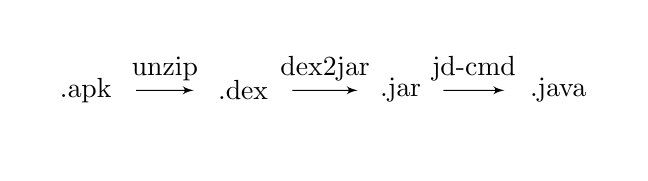
\begin{tikzpicture}[node distance = 2cm, auto]
    % Place nodes
     \node [cloud] (init) {.apk};
     \node [cloud, right of=init] (dex) {.dex};
     \node [cloud, right of=dex] (jar) {.jar};
     \node [cloud, right of=jar] (java) {.java};

     \path [line] (init) -- node {unzip}(dex);
     \path [line] (dex) -- node {dex2jar}(jar);
     \path [line] (jar) -- node {jd-cmd}(java);

\end{tikzpicture}
\caption{APK Extraction Process}
\label{fig:extractionprocess}
\end{center}
\end{figure}

%\vspace{-3 mm}

%% Reword how I am saying this since it is right out of the security paper
While no reverse engineering process can ever be considered perfect, our utilized technique has been demonstrated to be highly effective in previous research~\cite{apvrille2012android,chawla2014transfiguring, krutz2015FDroid, Lee_2013}. We also checked the accuracy of this reverse engineering process by manually analyzing at least 10 .java files from over 50 reverse engineered Android apps in our study. Since we used an already established reverse engineering process, there were few unforeseen hurdles in our collection or reverse engineering process.


\subsection{Step 3. Execute static analysis tools}
\label{sec: analysis}

The next phase was to analyze the extracted source code for a variety of metrics, including potential security risks, permissions issues, potential defects, and misuse of coding standards. We used the following tools for our analysis: %We also collected information about software clones, which are functionally equivalent portions of an application that may differ syntactically. A sign of poorly written software, clones may be detrimental to an application in a variety of ways, including increased maintenance costs and inconsistent bug fixes~\cite{Roy:2009:CEC:1530898.1531101}.

 \textbf{Stowaway:} Reports the over-permissions and under-permissions of an application, which we recorded. Similar to previous work~\cite{6624000}, we made slight modifications to Stowaway to accommodate our process and stay current with updated Android permissions. %%% Should I say something more about this?


 %Permlyzer~\cite{6698893}, a more modern permission detection tool, was not used since its authors have not made it available for download.

 \textbf{Androrisk:} Reports the security risk level of an application, which we recorded for every APK. Androrisk determines the security risk level by evaluating several criteria. The first is the presence of permissions which are deemed to be more dangerous. These include the ability to access the internet, manipulate SMS messages, or the rights to make a payment. The second is the presence of more dangerous sets of functionality in the app including a shared library, use of cryptographic functions, and the presence of the reflection API.



 \textbf{CheckStyle:} Measures how well developers adhere to coding standards such as annotation usage, size violations, and empty block checks. We recorded the total number of violations of these standards. Default application settings for Android were used in our analysis. While adherence to coding standards may seem to be a trite thing to measure, compliance to coding standards in software development can enhance team communication, reduce program errors and improve code quality~\cite{Li:2005:ETC:1095714.1095770, li2006using}.


 \textbf{Jlint:} Examines java code to find bugs, inconsistencies, and synchronization problems by conducting a data flow analysis and building lock graphs. We recorded the total number of discovered bugs. This tool was selected over FindBugs since it was able to analyze the applications much faster, while still providing accurate results~\cite{rutar2004comparison}.

 \textbf{APKParser:} A tool designed to read various information from Android APK files including the version, intents, and requested permissions.

We also recorded other metrics about each application including total lines of code, number of java files, application version, target SDK, and minimum SDK.


Stowaway and Androrisk were able to analyze the raw APK files, while CheckStyle, Jlint, and Nicad required the APK files to be decompiled. All results were recorded in an SQLite database, which is publicly available on the project website. The full analysis process is shown in Figure~\ref{fig:analysisprocess}.

\begin{figure}[h]
\begin{center}

% Define block styles
\tikzstyle{line} = [draw, -latex']

%\tikzstyle{cloud} = [draw, ellipse,fill=white!20, node distance=1.5cm, minimum height=2em]
\tikzstyle{cloud} = [draw=none, ellipse,fill=white!20, node distance=1.5cm, minimum height=2em]

\tikzstyle{block} = [rectangle, draw, fill=white!20, text width=5em, text centered, rounded corners, minimum height=4em]
\tikzstyle{c} = [draw, cylinder, shape border rotate=90, aspect=0.75, minimum height=70, minimum width=30]

\begin{tikzpicture}[node distance = 1.5cm, auto]

    % Place nodes
     \node [cloud] (init) {APK Collection};
     \node [block, below of=init] (ApkFiles) {ApkFiles};
     \node [cloud, below of=ApkFiles] (Decompile) {Decompile};
     \node [block, below of=Decompile] (DecompiledFiles) {Decompiled Files};
     \node [cloud, below of=DecompiledFiles] (JavaAnalysis) {Java Analysis};
    % \node [cloud, right of=ApkFiles] (apkanalysis) {Stowaway Androrisk};
    % \node [c, right of=DecompiledFiles] (SqliteDB) {SqliteDB};
     \node[c] (SqliteDB) [below right=-1.0cm and 2.4cm of DecompiledFiles]{SQLiteDB};

    \node[cloud] (apkanalysis) [below right=-0.9cm and 2.0cm of ApkFiles]
       {APK Analysis};

    % Draw edges
    \path [line] (init) -- (ApkFiles);
    \path [line] (ApkFiles) -- (Decompile);
    \path [line] (Decompile) -- (DecompiledFiles);
    \path [line] (DecompiledFiles) -- (JavaAnalysis);
    \path [line] (ApkFiles) -- (apkanalysis);
    \path [line] (apkanalysis) -- (SqliteDB);
    \path [line] (JavaAnalysis) -- (SqliteDB);
    \path [line] (Decompile) -- (SqliteDB);

\end{tikzpicture}
\caption{APK Analysis Process}
\label{fig:analysisprocess}
\end{center}
\end{figure}




\section{Evaluation}
\label{sec: evaluation}

In the following sections, we describe our findings based on our analysis and answer our research questions.

\subsection{RQX: How do app genres compare in terms of quality metrics?}

Android apps are separated into different groups known as categories or genres, some of which include `Communication', `Education', `Lifestyle', `Puzzle' and `Tools'. These different app groups all have different focuses, likely different target audiences, and very often different developers. We sought to better understand how apps from different genres compare against each other based on several metrics including coding standards issues, use of permissions, rate of under \& over-permissions, and app size. Table \ref{Table:topGroups} shows the top 10 collected categories, and an aggregate of all collected apps from Google Play (not just from the top categories) along with malicious apps.

%% Categories closely align (but do not perfectly match) the categories on http://www.appbrain.com/stats/android-market-app-categories

\begin{table*}
%% I removed JLINT coding standards from this table since the results were not that profound.
\begin{center}
\caption{Comparison of Groups}
\label{Table:topGroups}
 \begin{tabular}{ | l | c | c | c | c | c |  c |} \hline

  \bfseries Group & \bfseries LOC & \bfseries CS Mistakes/LOC & \bfseries Over-Permissions & \bfseries Under-Permissions & \bfseries Requested Permissions    \\ \hline

 	\bfseries Arcade &	152,563	 &	.01048 &	2.3 &	3.8 &	6.6 \\ \hline
 	\bfseries Books \& Reference &	123,600	 &	.00675 &	2.6 &	2.7 &	5.4 \\ \hline
	\bfseries Casual &	150,396 &		.0103~~ &	2.2 &	4 &	6.5 \\ \hline
 	\bfseries Communication & 	166,083  &	.06824 &	5.2 &	3.6 &	14.6 \\ \hline
	\bfseries Education &	131,615 &	.0234~~ &	2.2 &	3.3 &	5.8 \\ \hline
 	\bfseries Entertainment &	138,229 &	.01367 &	2.6 &	2.8 &	6.3 \\ \hline
 	\bfseries Lifestyle &	166,114 & 	.02639 &	2.9 &	3 &	8.2 \\ \hline
 	\bfseries Music \& Audio &	146,211	 &	.00985 &	2.5 &	2.7 &	6.7 \\ \hline
  	\bfseries Personalization &	113,539	  & 	.06075 &	3.8 &	2.5 &	8.3 \\ \hline
 	\bfseries Puzzle &	142,998 & 	.01025 &	2 &	3.8 & 	5.6 \\ \hline
	\bfseries Tools	 & 106,131 &	.07202 &	4.1 &	2.9 &	8.4 \\ \hline \hline
	
	%%% Version with JLINT
%	\bfseries Arcade &	152,563	& .0027 &	.01048 &	2.3 &	3.8 &	6.6 \\ \hline
% 	\bfseries Books \& Reference &	123,600	& .0025 &	.00675 &	2.6 &	2.7 &	5.4 \\ \hline
%	\bfseries Casual &	150,396 &	.0026 &	.0103~~ &	2.2 &	4 &	6.5 \\ \hline
% 	\bfseries Communication & 	166,083 &	.0029 &	.06824 &	5.2 &	3.6 &	14.6 \\ \hline
%	\bfseries Education &	131,615 &	.0023 &	.0234~~ &	2.2 &	3.3 &	5.8 \\ \hline
% 	\bfseries Entertainment &	138,229 &	.0024 &	.01367 &	2.6 &	2.8 &	6.3 \\ \hline
% 	\bfseries Lifestyle &	166,114 & .0023 &	.02639 &	2.9 &	3 &	8.2 \\ \hline
% 	\bfseries Music \& Audio &	146,211	 & .0025 &	.00985 &	2.5 &	2.7 &	6.7 \\ \hline
%  	\bfseries Personalization &	113,539	 & .0024 & 	.06075 &	3.8 &	2.5 &	8.3 \\ \hline
% 	\bfseries Puzzle &	142,998 & .0025 &	.01025 &	2 &	3.8 & 	5.6 \\ \hline
%	\bfseries Tools	 & 106,131 &	.0025 &	.07202 &	4.1 &	2.9 &	8.4 \\ \hline
	
	\bfseries Avg Google Play	 & 158,689 & .03065 & 3.0 &	3.3 &	7.8 \\ \hline
	\bfseries Malware	 & 32,373 & .06867 & 6 &	1.9 &	 12.4 \\ \hline
	
	
  \end{tabular}
  \end{center}
\end{table*}



%% I took out Jlint issues since these value were not all that surprising
%%We next analyzed the rate of discovered defects in each app by dividing the number errors detect by Jlint by the app's LOC. Surprisingly, we found that there wasn't a significant difference in the number of discovered defects which ranged from .0023/LOC-.0029/LOC. There are several possible explanations for these similar values. One is that since a large portion of

Adhering to proper coding standards is important for software development since it has been shown to have a variety of benefits including aiding team communication, increasing code quality and elevating overall application quality~\cite{Li:2005:ETC:1095714.1095770}. We measured the adherence to coding standards for each genre by dividing the number of coding standards mistakes discovered by CheckStyle by the LOC in the app. We found that there was a reasonably large variation of the amount of coding standards mistakes for genres with `Tools' having the most mistakes with .072 mistakes/LOC and `Books \& Reference' apps having the least with .00675 mistakes/LOC. While this may not seem like a large variation, the average LOC for all collected apps was 156,515, meaning that `Tools' apps would have an average of 10,212 more coding standards defects per app. Across the genres, we did not find a significant difference in the number of possible defects identified by Jlint.

We did find a large variation in the rate of over-permissions for each genre with `Casual' apps having the fewest with 2.2 per app and `Communication' having the largest with 5.2 for each app. `Personalization' apps had the fewest number of under-permissions (2.5), while `Casual' apps had the highest rate with 4 per app. `Lifestyle' apps were narrowly the largest with an average 166,114 LOC per app, while `Tools' apps were the smallest with 106,131 LOC. \\

\noindent
\textbf{Analysis}

%\todo{make sure M apps are introduced before this}
These findings are useful for a variety of reasons. The results show a wide disparity among the various categories in terms of app size, quality and security concerns. Developers may use this information to determine the concerns which require the most attention from a quality and security perspective. These results are important to researchers since it further demonstrates that app categories are not equal, and the possible relationships between quality and security in each of these categories.

over-permissions are a possible security vulnerability, so app categories with more over-permissions should be given more focus from security researchers from both the perspective of why they occur, to what their negative implications may be for these categories. With the introduction of Android 6.0, future work should be done to examine the rate of change in over-permissions in the different categories with this new permissions model. Also, since over-permissions are often caused by lack of developer understanding with the abused permissions~\cite{6624000}, these categories with the most over-permissions require the most developer education.

Due to the significant differences between several of the categories, further work should be conducted to determine why certain categories are more successful from a quality or security perspective. A few basic research questions for this potential study include if the development processes vary for these different categories, if organizations place different emphasis on app categories in terms of quality control, or even a potential impact of developer experience, and if there are different quality control metrics put into place for each of these categories. The results could be attained from developer interviews, and the analysis of open source Android app version control systems such as F-Droid to examine developer commits and app versions.

We also compared the averages of all collected apps from Google Play (not just those in our table) and compared these averages, against those from the malware apps. These results will be much further discussed later in the work.


%%% Briefly talk about the difference in Avg Google Play vs Malware, but remember that we will also focus on that later on



%Since lack of adherence to coding standards and apps with too many, or too few permissions are indications of developer's not being diligent about the quality of the apps, we next checked to see if there was a correlation between lack of adherence to coding standards and over \& under privileges. \todo{how to best do this correlation?}

%\todo{What more can we learn from these comparisons?}

% Is there a correlation between coding standards and rates of Over and under privs?


%%% Show some kind of chart


\subsection{RQX: What are the most pervasive over-permissions?}

A basic security principle is the concept of granting of the least amount of privileges to an application that it needs to properly function. Granting extra privileges creates unnecessary security vulnerabilities by allowing malware to abuse these unused permissions, even in benign apps. These extra privileges also needlessly increase the app's attack surface~\cite{Davi:2010:PEA:1949317.1949356, Bartel:2012:ASP:2351676.2351722}. Previous research has found that while Android developers often add extra privileges to make the app work properly, or due to confusion over the permission name, they often add them unnecessarily believing its functionality sounds related to their app~\cite{Felt:2011:APD:2046707.2046779}. We analyzed the most overused permissions for all apps and present the ten most commonly occurring over-permissions in Table \ref{Table:topOverPrivs}. \\

%% Considered adding malware into this, but did not since I wanted to keep the focus on GP apps.

\begin{table}[]
\begin{center}
\caption{Top Occurring over-permissions in GP Apps}
\label{Table:topOverPrivs}
 \begin{tabular}{ | l | c | } \hline

  \bfseries Permission & \bfseries Rate  \% \\ \hline
	
	GET\_ACCOUNTS  & 10 \\ \hline
	READ\_EXTERNAL\_STORAGE & 9 \\ \hline
	CALL\_PHONE  & 7 \\ \hline
	ACCESS\_WIFI\_STATE & 7 \\ \hline
	SYSTEM\_ALERT\_WINDOW & 6 \\ \hline
	READ\_PHONE\_STATE  & 6 \\ \hline
	WRITE\_EXTERNAL\_STORAGE  & 4 \\ \hline
	WRITE\_CONTACTS  & 4 \\ \hline
	GET\_TASKS & 4 \\ \hline
	CHANGE\_NETWORK\_STATE  & 4 \\ \hline
	 	
  \end{tabular}
\end{center}
\end{table}



\noindent
\textbf{Analysis}

\todo{add more to this}

%%% Why is this really importat? Why should people care?


These top occurring over-permissions can be dangerous for a variety of reasons. For example,~\texttt{GET\_ACCOUNTS}, permits access to the list of accounts in the accounts service,~\texttt{READ\_EXTERNAL\_STORAGE}, allows the application to read from an external storage device and \texttt{CALL\_PHONE}, allows an app to start a phone call without the user confirming it through the dialer interface~\cite{manifest_url}.

Research has shown that developers typically abuse permissions due to not properly understanding it, and that developer education and community support is paramount for eliminating permission abuse~\cite{6624000}. Based on our observations, we believe that these ten permissions require the most attention and education in order to reduce their rate of abuse.

All of the apps we analyzed were Android version \textless 6.0, and therefore did not use the new Android permission structure which permits apps to ask for permissions at runtime. Future work could be conducted to examine the possible implications of this new permission structure on app over-permissions. From a technical perspective, will the new version of Android reduce the number of over-permissions, and will developers pay more or less attention now to possible app over-permissions?

%Updates to the Android OS often contain changes to the permissions options available to developers. These changes could be relatively simple where new permissions are made available in a release update, to being as profound as the permissions overhaul conducted in Android 6.0. Over the last few years, there has been large amount of research conducted on how to improve the Android permissions model. Some of these updates range from the \todo{xxxxx}.

%Our results about permissions usage and over-permissions could prove to be invaluable


There has been a large amount of research on how to improve Android's permission structure ranging from a increasing user understanding~\cite{Sarma:2012:APP:2295136.2295141} to increasing security through the use of more fine grain permissions~\cite{jeon2011dr}.\todo{finish}


% Overprivileged applications expose users to unnecessary permission warnings and increase the impact of a bug or vulnerability {Android Permissions Demystified}

% 

%%% Knowing 

%%%  

\todo{Look into this more...}

? If an app was granted permission, could another malicious app (signed using the same key) maliciously use that permission?



Felt~\emph{et al.}~\cite{Felt:2011:APD:2046707.2046779} suggested that developers frequently mistakenly request permissions with names which sound like their app's functionality. They found that only 32\% of the apps which request~\texttt{ACCESS\_WIFI\_STATE} actually need WiFi permissions, and that they most often only need network access. Our findings further demonstrate continued clarification and attention to these areas.\dan{clean up}



%%% If true -> These frequently occurring overprivs are also important for 

%% Curtailing Privilege Escalation Attacks over Asynchronous Channels on Android
%Moreover we believe that the real threat is what we coined
%insidious trustfulness pretension. An attacker can
%create a useful and successfully operating App which is widely
%accepted and top-rated by the community. Therefore this App
%helps establishing the developer�s trust to the community.
%If a second, now malicious App is created by the same
%App developer, the attacker can insidiously profit from his
%reputation since the new App will at least tried out by the
%trusting user base. This is also true for updates of previously
%installed and accepted Apps.

%Such an App could be a task scheduling App which
%synchronizes to a web server. It would only need INTERNET
%permission. When this malicious App is also installed on the
%target device running the SMS FORMATTER, it can effortlessly
%access all data. If the formatter exchanges data with its stand-
%alone widget by using Intents, the task scheduler can request
%SMS data by Intents too.





% What do other over priv works say about improving the permssions modeling based on knowing overprivs
%


%Since Android's inception, there have been large amounts of research on how to improve the Android permission model. The recommendations range from .... to .... .  \todo{how can our information be used to improve the permissions model}
\todo{intents, IPC?} % Go back and read about the Android vulnerability readings

%%%% How can intents, the IPC misuse these areas?








%%% Maybe add a bit more to this


\subsection{RQX: Is there a correlation between quality \& security?}
%%% New section

When developing software, there are several primary concerns of developers, two of which include the security and the quality of the application. We next sought to determine if there was typically a correlation between the security of an application, and its quality. We measured quality by adherence to coding standards (Checkstyle) and detected possible bugs (Jlint), while security was measured by the Androrisk score and number of detected over-permissions. Both Jlint and Checkstyle values were normalized by the app's LOC to limit the effects of an app's size on the results.

We used the Spearman rho and Kendall correlation metrics to determine if there was a correlation between quality and security. When using the Spearman rho and Kendall correlation metrics, the correlation coefficient will vary between -1 and +1. As the value of the coefficient approaches $\pm$1, there is more of a monotonic, or perfect degree of association between the evaluated values. The relationship between the evaluated values becomes weaker as the correlation coefficient approaches 0. Using these correlation metrics, we evaluated the relationship strength of quality (Coding Standards Defects \& Jlint Errors) and security (Androrisk \& over-permissions). The results of this analysis are shown in Table~\ref{table:appCorrelationMetrics}.


%%% Do a correlation between CS and Jlint

\begin{table}[h]
\centering
\caption{Correlation Metrics for Quality \& Security}
  \begin{tabular}{ | c | c || c | c | c |  } \hline \hline
  	\multicolumn{2}{ | c |  }{\bfseries Area}  & \multicolumn{2}{ | c |  }{\bfseries Correlation} \\ \hline

	%[1] "OPriv: Jlint: 0.182495980050052 K: 0.137639881834338"
	%[1] "OPriv: CSDefect: 0.125835596829345 K: 0.10127868061073"
	%[1] "FuzzyRisk: CSDefect: 0.14304868296507 K: 0.114805274418005"
	%[1] "FuzzyRisk: JlintResult: 0.385023458032465 K: 0.294240150104432"


   	\bfseries Security  & \bfseries Quality & \bfseries  Spearman  &   \bfseries   Kendall  \\ \hline \hline
    	OPriv  & Jlint &  .18249 & .13764   \\ \hline
    	OPriv  & CSDefect &  .12584  & .10128   \\ \hline
    	Androrisk  & CSDefect &  .14305 & .11481   \\ \hline
    	Androrisk  & Jlint &  .38502 & .29424   \\ \hline
%	CSDefect  & Jlint &  .53095 & .41133   \\ \hline % Could show this, but not securty & quality. Ruins headers

  \end{tabular}
\label{table:appCorrelationMetrics}
\end{table}



\noindent
\textbf{Analysis}
\dan{check everything below for accuracy}
%% Maybe find some newer links



%%% I think that contradicting other findings may be dangerous for our work
Based on our analysis, we found only a weak association between the quality and security of applications in the several evaluated comparisons. This indicates that there is no significant correlation between the security and quality of an app. These findings are somewhat surprising since previous research has discussed the importance of adhering to coding standards as a way for developers to avoid mistakes and improve overall application security~\cite{embeddedSecurity_url, Kleidermacher:2012:ESS:2222505}. Our findings demonstrate the need for further research and analysis in this area.

%We also compared two quality attributes, Checkstyle defects and Jlint issues and found a somewhat stronger, but still fairly weak association between the two.
%% Not sure I should discuss this....



% How is this information useful? What can be done with it? What is the novelty of this?



\todo{add more to this. See if more papers can be found in this area}
% http://www.embedded.com/design/safety-and-security/4418986/Using-coding-standards-to-improve-software-quality-and-security

% http://www.continuitycentral.com/news07337.html - maybe?







%%%%%% ^^^^^^^^^^^^^^^^^^^^^^^^^^^^^^^^^^^^^^^^^^^^^^^^^^^^^^^

\subsection{RQX: How do benign \& malicious Android apps compare in terms of quality?}


% Fortinet.com,. 'Fortinet?S Fortiguard Labs Reports 96.5% Of All Mobile Malware Tracked Is Android Based, Symbian Is Distant Second At 3.45%; Ios, Blackberry, Palmos, And Windows Together Represent Less Than 1%Fortinet | Network Security, Enterprise And Data-Center Firewall'. N.p., 2014. Web. 10 July 2014.

In 2013 alone, there were at least 1,800 new mobile malware families, with over 96\% of malware targeting Android~\cite{Fortinet_url}. Despite protection measures taken by Google such as Bouncer, malware continues to be a significant problem by using sophisticated mechanisms to evade detection.~\cite{Kate:2015:TPS:2791405.2791558}.


In order to better understand Android malware, we compared the static analysis results from apps collected from the Google Play store against 1,417 malware examples taken from the Contagio Mobile Mini Dump~\cite{contagio_url} and the Malware Genome Project~\cite{Zhou:2012:DAM:2310656.2310710}. We chose to evaluate the malware samples against those collected from Google Play in a variety of areas including Androrisk score, adherence to coding standards, discovered potential defects, over \& under-permissions, and the requested app permissions. The results of this analysis are available on our website and are shown at the bottom of Table~\ref{Table:topGroups}.

%This was accomplished by running the malicious applications through the same process as the applications collected from the Google Play store, described in Sections~\ref{sec: decompliation} and~\ref{sec: analysis}. \todo{describe what each of the sets of data mean}


%%% Removed since the values are very similar to what is in the large table. I felt like it was redundant info
%\begin{table}[h]
%\begin{center}
%\caption{Averages for Malware vs. Non-Malicious}
%\label{Table:maliciousvsnonmalicious}
%  \begin{tabular}{ | l | c | c | } \hline
%
%     \bfseries Analysis Value  & \bfseries Malicious & \bfseries Google Play \\ \hline
%
%
%   % Avg. LOC /App & 30,547 & 156,515. \\ \hline   % Not sure this is a great stat to show
%    Jlint Errors/LOC & 0.00298 & 0.00256 \\ \hline
%    Coding Standard Mistakes/LOC & 0.069 & 0.031 \\ \hline
%    over-permissions/App & 6.0 & 3.0 \\ \hline
%    under-permissions/App & 1.9 & 3.3 \\ \hline
%    Permissions/App & 12.4 & 7.8 \\ \hline
%%    Opriv/Priv\dan{remove?} & 2.06 & 2.57 \\ \hline
%%    Upriv/Priv\dan{remove?} & 6.86 & 2.41 \\ \hline
%	Androrisk & 56.95 & 63.28 \\ \hline
%
%  \end{tabular}
%  \end{center}
%\end{table}



%%% Should I instead say threshold?
\todo{Add in Spearman?}
\hl{After collecting the above results we next tested the statistical significance of our findings using the one tailed Mann Whitney U (MWU) test for the hypothesis testing, since it is non-parametric and we can find out if the low-rated apps indeed have higher or lower values for each of the security metrics. The MWU test compares two population means that originate from the same population set and is used to determine if two population means are equal. A P value which is smaller than the significance level implies that the null hypothesis can be rejected. Conversely, a P value which is equal to or greater signifies that the null hypothesis cannot be rejected. In our analysis, we used a threshold of .05 to determine if we have enough data to make a decision if the null hypothesis should be rejected.} As shown Table~\ref{table:studyresultsMWU}, the results of this analysis further validate our findings displayed in Table~\ref{Table:topGroups}.

%%% Mention that there is no difference between
%% \checkmark
\begin{table}[h]
\centering
\caption{MWU Results for Malicious \& Benign apps}
  \begin{tabular}{ | l | c | c | c | c |  } \hline
    % \bfseries Genre  & \bfseries \% of Apps \\ \hline

 & \multicolumn{2}{ c |  }{\bfseries Greater In}   & \\ \hline
    \bfseries Area  &  \bfseries  Malware &  \bfseries   GP & \bfseries P-value\\ \hline \hline

% Use \checkmark

       % Item  & X & X & X \\ \hline

	Jlint Errors/LOC  & \checkmark & &  4.7587e-09 \\ \hline
    	Coding Standard Mistakes/LOC  & \checkmark &  &  7.8306e-110 \\ \hline
    	Over-permissions/App  & \checkmark & &  2.7002e-142 \\ \hline
    	Under-permissions/App  &  & \checkmark & 3.0972e-30 \\ \hline
    	Permissions/App  & \checkmark &  & 3.0872e-121 \\ \hline
    	Androrisk  &  & \checkmark & 2.1298e-32 \\ \hline

  \end{tabular}
\label{table:studyresultsMWU}
\end{table}




\noindent
\textbf{Analysis}


Based on our comparison of malicious apps compared to those from Google Play, we made several primary discoveries. The first is that \emph{Developers of Malware are not overly concerned with the quality of their apps:} Most Android malware is piggybacked on existing applications and malicious code is typically loosely coupled with the host application~\cite{Zhou:2012:DAM:2310656.2310710, Deshotels:2014:DAF:2556464.2556467}. We found that malicious applications had a much higher number of coding standards mistakes per LOC compared to their benign counterparts while also having a higher number of possible bugs discovered by Jlint per LOC. Although we are not able to examine the development process of malware applications or interview its developers, we are able to draw several possible conclusions. Malware developers likely care less about the actual user experience as they are not overly concerned with app quality or coding standards. This lack of attention to quality is also demonstrated by the number of over-permissions in malware compared to apps from Google Play.




%A threat to our findings is the possible affects which obfuscation tools could have in affecting our results. This was a significant concern we had, even from the beginning of our collection and analysis process.
\todo{?mention something about obfuscation?}

%% Randomly examined 100 of the reverse engineered apps and did not find any


under-permissions are a quality concern since an app will likely crash if it requests a permission which it was not granted. What is somewhat surprising is that malicious apps actually have fewer under-permissions per app compared to apps from Google Play. An explanation for this could merely be that the permissions in malicious apps are more often being used, unfortunately for disruptive activities.

\emph{Malicious apps request more permissions than benign apps:} Malicious apps request an average of 12.4 permissions compared with 7.8 permissions for those collected Google Play. Malware is more likely to request these additional permissions to perform malicious activities~\cite{Sarma:2012:APP:2295136.2295141}.


%%% Might be a good idea to remove this since we are not evaluating this tool and we use it in the paper
%We also found that \emph{Androrisk is not a good evaluator of determining if an app is malicious:} On average, malicious apps actually had a lower Androrisk score as compared to Google Play apps. This is a representative of the difficulties that static analysis tools have in detecting malware~\cite{4413008, Feng:2014:ASD:2635868.2635869} and should not be construed as a statement that Androrisk is any better or worse than any other static analysis tools. \dan{remove this if it is being used as a guideline in other areas}



%\todo{? Talk about how this could tie into the rest of the malware detection process?}

% Much higher rate of Jlint & Coding errors in malware vs. GP
% Many more overprivs in malware, but the ratio of overpriv/app privs is actually lower. This is likely due to malicious apps making use of all requested privs for malicous reasons. This is backed up by the fact that the ratio of Overprivs/requested privs is actually lower for maliciuos apps.


% Red flags for malicious applications
% Demonstrates what malicious users like to do
% Read other papers to see what they say about permissions

%%% These values changed a bit for our most recent analysis
%%% Might not be a bad idea to run them once more



\textbf{What are the most common permissions in Android malware?}

We next compared the requested permissions for all malicious and benign apps using a custom-built permissions extraction tool. The primary difference between requested permissions and over-permissions is that requested permissions are merely those that the app asks to use, and does not take into consideration if the app actually needs them or not.

We compared the top ten rates of requested permissions for the malicious apps against those recorded from Google Play. The results of this comparison are shown in Table~\ref{Table:permissions_usage}. The Android Malware Repository\footnote{\url{https://sites.google.com/site/androidmalrepo/permission-stats}} used a different malware oracle and found similar permissions results to what we discovered, which provides confidence to our findings. Unfortunately, they do not appear to have analyzed any apps since 2012.


%We next analyzed all 1,417 malware samples and recorded the permissions each app requested. Since the requested permissions for each app are stored in its~\emph{AndroidManifest.xml} file, we built an extraction tool to record these requested permissions. The primary difference between requested permissions and over-permissions is that requested permissions are merely those that the app asks to use, and does not take into consideration if the app actually needs them or not.



% We performed the same process on the 31,234 apps from Google Play and compared the top ten rates of requested permissions for the malicious apps against those recorded from Google Play. The results of this comparison are shown in Table~\ref{Table:permissions_usage}. The Android Malware Repository\footnote{\url{https://sites.google.com/site/androidmalrepo/permission-stats}} used a different malware oracle and found similar permissions results to what we discovered, which provides confidence to our findings. Unfortunately, they do not appear to have analyzed any apps since 2012.


\begin{table}[h]
\caption{Permissions Usage}
\label{Table:permissions_usage}
 \begin{tabular}{ | l | c | c | } \hline

  \bfseries Permission & \bfseries Malware \%& \bfseries G-Play \%\\ \hline

	INTERNET	& 98 &	94 \\ \hline
	READ\_PHONE\_STATE	& 93 &	45 \\ \hline
	ACCESS\_NETWORK\_STATE	 & 81 &	84 \\ \hline
	WRITE\_EXTERNAL\_STORAGE &	68 &	62 \\ \hline
	ACCESS\_WIFI\_STATE &	61 &	36 \\ \hline
	READ\_SMS &	60 & 	4 \\ \hline
	RECEIVE\_BOOT\_COMPLETED &	56 & 1 \\ \hline
	WRITE\_SMS &	49 &	2 \\ \hline
	SEND\_SMS &	45 &	4 \\ \hline
	RECEIVE\_SMS &	42 &	5 \\ \hline

%%% To find this I found the top privs in malware and found the correlating values for Google Play

  \end{tabular}
\end{table}

\noindent
\textbf{Analysis}


%\todo{more granularity} % Should these heavily used permissions have more granularity? See what was done for 6.0

While most apps from each group request \texttt{INTERNET} and \newline \texttt{ACCESS\_NETWORK\_STATE},  we found that malicious apps requested a disproportionately high number of other permissions. 93\% of malicious apps requested~\texttt{READ\_PHONE\_STATE}, which is more than twice the average for Google Play apps. This permission is particularly dangerous since it provides the app access to a wide variety of information and functionality including verifying the user's phone with IMEI information and gathering personal information such as your phone number.

Malicious apps also requested a much higher rate of SMS related permissions including \texttt{READ\_SMS}, \texttt{WRITE\_SMS}, \texttt{SEND\_SMS} and \texttt{RECEIVE\_SMS}. Malware often propagates to other devices through SMS messages. One such example of this is~\emph{Selfmite}~\cite{zorz_zeljka_aggressive_2014}, which is an Android worm that spreads through SMS messages. SMS systems may also be abused by sending premium rate SMS messages, which could likely go unnoticed until the user receives and examines their next bill~\cite{felt2011survey}.


\texttt{RECEIVE\_BOOT\_COMPLETED} is requested 56\% of the time by malicious apps compared with only 1\% for GoogePlay apps. This permission is often used by malware to notify it that the phone has been rebooted allowing it to begin installing malicious services~\cite{canfora2013classifier}.

Malicious apps request \texttt{ACCESS\_WIFI\_STATE} 61\% of the time compared to only 36\% for apps from Google Play. This permission allows apps to access several pieces of information related to the Wi-Fi interface including accessing a user's location. Unfortunately, malicious apps have used this permission to leak personal information about the user, including their location, which they often sell to advertisers~\cite{achara2014wifileaks}.

The knowledge of what permissions have a higher prevalence in malware has several possible uses. Apps which request these permissions could be noted to have a higher probability that they are malicious. Since many benign apps have legitimate uses for these permissions, they cannot be the sole indicator, but can be an sign of a possibly malicious application. Understanding what permissions malware requests may be useful for understanding how current and future malware spreads and affects devices.

%We then examined the rates of over privileges in malicious apps compared to benign apps. The top 10 most commonly occurring over privileges, their rates, and how they differ from applications collected from the Google Play store, are shown in Table~\ref{Table:mal_permissions}.\todo{update analysis}
%\todo{keep this?}

%\begin{table}[t]
%\caption{Top Occurring over-permissions in Malware vs. Google Play\dan{Is this useful? I think it can be meaningful data, I am just not sure how to best analyze it.}}
%\label{Table:mal_permissions}
%  %\begin{tabular}{ | p{5.3cm} | p{1.0cm} | p{1.2cm} | } \hline
 %\begin{tabular}{ | l | c | c | } \hline

  %\bfseries Permission&\bfseries Malware \%&\bfseries G-Play \% \\ \hline

%	READ\_SMS	& 60.1	& 2.8 \\ \hline
%	WRITE\_SMS	& 49 &	1.7 \\ \hline
%	CALL\_PHONE	 & 30.3 &  6.3 \\ \hline
%	WRITE\_CONTACTS	& 28.2 &	3.6 \\ \hline
%	WRITE\_APN\_SETTINGS &	25 & .5 \\ \hline
%	ACCESS\_WIFI\_STATE	& 24 &	5.9 \\ \hline
%	WAKE\_LOCK	& 20	& 2.5 \\ \hline
%	RESTART\_PACKAGES &	15.6 &	1.4 \\ \hline
%	VIBRATE	& 13.9 &	1.6 \\ \hline
%	READ\_LOGS	& 13.8 &	1 \\ \hline
%  %%% Make sure that all values are to the same decimal point

%  \end{tabular}
%%% To find this I found the top overprivs in malware and found the correlating values for Google Play
%\end{table}

%\todo{talk about how this is useful}



%%%%%%%%%%%%%%%%%%%%%%%%%%%%%%%%%%%%%%%

We next conducted a small case study on several malicious Android apps collected from the Contagio Mobile Mini Dump. The first app we selected was a fake version of Netflix, which would collect the user's information when faking a login to the Netflix service. After reverse engineering this app, we found that some of its requested privileges included \texttt{ACCESS\_NETWORK\_STATE}, \texttt{READ\_PHONE\_STATE} and \texttt{ACCESS\_WIFI\_STATE}, which are all permissions which are much more likely to be requested by malware. We selected a sample known as `LoveTrap'~\cite{LoveTrap_url1} which was originally available in a third-party app store. Some of the app's requested permissions included \texttt{READ\_PHONE\_STATE}, \newline \texttt{RECEIVE\_BOOT\_COMPLETED}, \texttt{SEND\_SMS} and \texttt{RECEIVE\_SMS} which are all much more likely to appear in malware than in benign apps. The app used \texttt{RECEIVE\_BOOT\_COMPLETED} permission to execute itself once the infected Android device was rebooted, and used the SMS related permissions to subscribe to services which may lead to unwanted charges for the infected user.



For benign apps, our results support a possible need for a more granularly defined permission structure for the most requested permissions. Since these permissions are so frequently requested, further refinement of these permissions could increase the security level of an app by limiting overly broad access. This is something which is supported by previous research~\cite{jeon2011dr}. Android 6.0 has attempted to address this issue by \todo{finish }

%%% How has Android M handled this


%%% permissions leaks?




% Move this to be higher up?
%% Talk about the malicious things that would specific to this app?
%   Find URLs for each of these malicious apps
% ? Do the specific privs requested match up with what I found to be malicious?

%%% DK: 8/28 - Could not find Good fake version to use

%\todo{Added this next part in}
%We next performed a case study on several specific
%
%%% Mention how these are popular
%We next compared fake, malicious copies of `Netflix' and `Player' as identified by the Malware Genome Project. A single fake copy of Netflix was included, with six fake copies of Player. We ran these fake copies of the applications against legitimate versions attained from the GooglePlay store. In both instances, the fake versions of the applications were significantly smaller than their real counterparts. We chose to only report on the Fuzzy Risk, over privilege count, and number of Java files since many of the other results of the analysis were not deemed useful due to the small size of the fake applications. The Fuzzy risk value was similar for both versions of the Netflix applications, but the real version of the Player application had a significantly higher value than its fake counterpart. The number of overprivliledges was much higher for the Fake Netflix application compared
%
%
%Full results are shown in Table~\ref{Table:fakesvsRegular}.
%
%
%
%\begin{center}
%
%\begin{table}[ht]
%\caption{Fakes vs. Regular}
%\label{Table:fakesvsRegular}
%  \begin{tabular}{ l | l | l | l }
%
%    \bfseries Application  & \bfseries Fuzzy Risk  & \bfseries Over Privileges & \bfseries Java Files \\ \hline
%    Fake Netflix & 51 & 9 & 11 \\ \hline
%    Netflix & 50 & 2 & 2429 \\ \hline \hline
%    Fake Player (Avg) & 50 & 0 & 14 \\ \hline
%    Player & 92 & 0 & 813 \\
%  \end{tabular}
%\end{table}
%\end{center}
%
%
%%% Run MWU on these?





%%%%%% ^^^^^^^^^^^^^^^^^^^^^^^^^^^^^^^^^^^^^^^^^^^^^^^^^^^^^^^





\subsection{RQX: How are apps changing over time?}

We next compared how Android malware and Google Play apps are evolving on an annual basis in terms of size (LOC) and requested permissions. We separated the apps collected from the Contagio Mobile Mini Dump into those created in or before 2012, 2013, 2014, and 2015. The results of this analysis are shown in Figure~\ref{fig:malwareEvolutionLOC} and Figure~\ref{fig:malwareEvolutionPriv}. \\

% We did not use apps from the Malware Genome Project since we were unable to collect accurate date information for these apps. -- These were used


%%%% -----------
%% Colors used for bar chart
\definecolor{bblue}{HTML}{4F81BD}
\definecolor{ggreen}{HTML}{9BBB59}

\begin{figure}[h]
%\vspace{-0.05in}
\begin{tikzpicture}
\begin{axis}[
    ybar,
%	scale only axis,
    enlargelimits=0.15,
    legend style={at={(0.5,.9)},
      anchor=north,legend columns=-1},
      ylabel=LOC (100K),
%   ylabel={\#participants},
    symbolic x coords={$\leq $ 2012,2013,2014,2015},
    xtick=data,
%    nodes near coords,
%    nodes near coords align={vertical},
	xticklabel style={text width=4em, font=\small},
	bar width=12pt
    ]

%%% For LOC
%% Malware
\addplot [style={ggreen,pattern=north east lines,mark=none}]coordinates {($\leq $ 2012,17693.375)(2013,32988.662)(2014,7 4606.432)(2015,109947.075) };

%% GP
\addplot [style={bblue,pattern=dots,mark=none}]coordinates {($\leq $ 2012,35645)(2013,86482)(2014,181225)(2015,229355) };




\legend{Malware, Google Play}
\end{axis}
\end{tikzpicture}
\caption{Evolution of Apps - LOC}
\label{fig:malwareEvolutionLOC}
\end{figure}


%%% analyze the results

\begin{figure}[h]
%\vspace{-0.05in}
\begin{tikzpicture}
\begin{axis}[
    ybar,
%	scale only axis,
    enlargelimits=0.15,
    legend style={at={(0.5,.9)},
      anchor=north,legend columns=-1},
      ylabel=Requested Permissions,
%   ylabel={\#participants},
    symbolic x coords={$\leq $ 2012,2013,2014,2015},
    xtick=data,
%    nodes near coords,
%    nodes near coords align={vertical},
	xticklabel style={text width=4em, font=\small},
	bar width=12pt
    ]



%%% For Priv
%% Malware
\addplot [style={ggreen,pattern=north east lines,mark=none}]coordinates {($\leq $ 2012,7.8)(2013,10.7)(2014,13)(2015,18.2) };

%% GP
\addplot [style={bblue,pattern=dots,mark=none}]coordinates {($\leq $ 2012,4.61)(2013,6.3)(2014,8.3)(2015,8.9) };




\legend{Malware, Google Play}
\end{axis}
\end{tikzpicture}
\caption{Evolution of Apps - Permissions}
\label{fig:malwareEvolutionPriv}
\end{figure}



\noindent
\textbf{Analysis}

We found that malicious apps are growing on an annual basis in both LOC and requested permissions. An interesting discovery is that although both are consistently growing, Google Play apps are larger in terms of LOC, but are smaller in the number of requested permissions.

Our findings have several important implications for both general app development, and malware research. For developers of benign apps, indications are that apps will continue to grow in terms of LOC and in requested permissions. This is significant for several reasons. The first is that with more permissions, developers will need to be better educated about the permissions they use and diligent to ensure that they are properly using them. This will be further complicated by Google's move to a new permission structure in Android 6.0 which will allow apps to request permissions at runtime instead of only upon installation of the app.

Since apps are becoming larger in terms of LOC, this will likely mean that teamwork will becoming increasingly more important since more developers will be needed to create an maintain the apps. With more developers being involved in the app, fundamental software engineering skills such as communication, documentation, diverse team roles, testing and adhering to coding standards will become increasingly important~\cite{Pressman:2009:SEP:1593949}.

Although malware is on average smaller in terms of LOC in comparison to benign apps, malware is growing and requesting more permissions on an annual basis. There are a variety of current malware detection techniques including API tracing~\cite{6298136}, behavioral based techniques~\cite{burguera2011crowdroid, shabtai2012andromaly}, and permission based systems~\cite{talha2015apk}. A popular method of discovering malware is a signature based approach where static analysis tools examine applications for known virus patterns~\cite{Feng:2014:ASD:2635868.2635869}. Larger software will make many of these processes more difficult and time consuming, leading for the need for different and more efficient processes.

Malware is also growing in terms of requested permissions. We next examined which permissions were being added to malware at the fastest rate. We began by counting all requested permissions for malware created in 2012, 2013, 2014, and 2015. We then calculated the frequency that each permission was requested. Figure~\ref{fig:malPermissionGrowth} shows the rate of change in the top 4 most prominent permissions requested in our malware collection.

% Although we observed that there several permissions whose usage became much more prominent in even only a 3 year span, we saw that there was a more general, more moderate growth among utilized permissions on an annual basis. \todo{.3?}

% Good site
% http://tex.stackexchange.com/questions/134346/different-marker-shape-for-pgf-tikz
\begin{figure}
\begin{center}

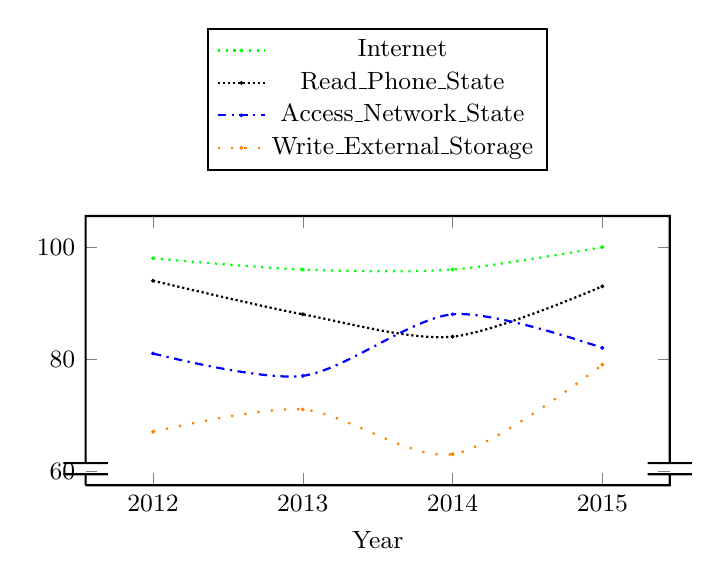
\begin{tikzpicture}
\begin{axis}[
   smooth,
   width=9cm,
   height=5cm,
   enlargelimits=0.15,
  xlabel={Year},
  %ylabel={\%},%% Takes up too much room
  symbolic x coords={2012, 2013,2014,2015},
  xtick=data,
  x tick label style={rotate=0,anchor=north},
% legend pos=north west, % original
  %legend pos=south east,
  legend style={at={(0.5,1.7)},anchor=north},
  font=\small, ,line width=.8pt,mark size=.2pt,
 axis y discontinuity=parallel,
]

% Defects - Jlint
\addplot [color=green,dotted,mark=*,mark options={solid},smooth] plot coordinates {(2012, 98) (2013,96) (2014,96) (2015,100) };
\addlegendentry{Internet}

\addplot [color=black,densely dotted,mark=*,mark options={solid},smooth] plot coordinates {(2012, 94) (2013,88) (2014,84) (2015,93)};
\addlegendentry{Read\_Phone\_State}

\addplot [color=blue,dashdotted,mark=*,mark options={solid},smooth] plot coordinates {(2012, 81) (2013,77) (2014,88) (2015,82)};
\addlegendentry{Access\_Network\_State}

\addplot [color=orange,loosely dotted,mark=*,mark options={solid},smooth] plot coordinates {(2012, 67) (2013,71) (2014,63) (2015,79)};
\addlegendentry{Write\_External\_Storage}


%%% Removed since it was so off
%\addplot [color=red,dashed,mark=*,mark options={solid},smooth] plot coordinates {(2012,64) (2013,28) (2014,53) (2015,68)};
%\addlegendentry{Access\_Wifi\_State}

\end{axis}
\end{tikzpicture}
\end{center}
\caption{Malware Permission Growth} \label{fig:malPermissionGrowth}
\end{figure}

As indicated by the chart, while there may be a general upward movement in the requested permission frequency for these permissions, the trend is not consistent. \todo{significance to this?} We next chose to examine the usage rate in several of the permission requests which were growing at the most substantial rate between 2012 and 2015 in malware. The results of this are shown in Table~\ref{Table:malPrivGrowth}.


\begin{table}[ht]
\begin{center}
\caption{Malware Permission Growth By Year}
\label{Table:malPrivGrowth}
 \begin{tabular}{ | l | c | c | c | c |} \hline

& \multicolumn{4}{ c | }{\bfseries \% Occuring} \\ \hline
	  \bfseries Permission & \bfseries   2012 & \bfseries 2013  & \bfseries 2014 & \bfseries 2015 \\ \hline %\hline

	RECEIVE\_BOOT\_COMPLETED & 55 & 52 & 71& 86 \\ \hline
	READ\_CONTACTS & 36 & 55&  41& 68 \\ \hline
	SYSTEM\_ALERT\_WINDOW &1 & 16 &  27 & 61 \\ \hline
	WAKE\_LOCK &34 & 19 & 41 &54 \\ \hline
	GET\_TASKS &17 & 25 & 43 & 39 \\ \hline	
	%MOUNT\_UNMOUNT\_FILESYSTEMS & 10 & 19 & 14 & 32 \\ \hline

  \end{tabular}
\end{center}
\end{table}

These results indicate that malware is using these permissions much more frequently now, than even a few years ago. For instance, the usage of \texttt{SYSTEM\_ALERT\_WINDOW} has gone from appearing in 1\% of malware in 2012, to 61\% in 2015. This permission allows an an app to create new windows on the Android UI, and may often be used by malware to display a message in an attempt to convey misinformation to the user. Security researchers can analyze these trends to see how malware is evolving over time and the different types of attacks they are attempting to perform using these extra permissions. This information could prove to be invaluable for both detecting and countering the negative effects of malware.

The new Android 6.0 permissions model substantially changed both how app permissions are requested, along with how many permissions are categorized (normal or dangerous). For example, the \texttt{INTERNET} permission previously required a user's authorization for an app's use, however in Android 6.0 it is defined as a 'Normal' permission, meaning it does not require a user's authorization. Understanding the permission trends in malware is paramount for understanding any further adjustments which are required to any updated permissions model. Possible alterations could include the further consolidations for permissions and their groups, adjustment of `Normal' and `Dangerous'  permission groups, or even the creation of new permissions.

Although there should be further analysis of Android 6.0 malware before any definitive recommendations are made, it is concerning that three of the top 10 most requested malware permissions of 2015 (\texttt{INTERNET}, \texttt{ACCESS\_NETWORK\_STATE} and \\ \texttt{ACCESS\_WIFI\_STATE}) are considered to be `Normal' permissions in Android 6.0, meaning the user will not be prompted to give the app access to these permissions.






%%% Could this information be used to determine how malware is attacking things? Reorganize permission models?





%\todo{add more analysis about the growth of these items}

%%% Do some work to discover more information about android malware
%
%
%% The possible reasons for the growth in these requested permissions is quite numerous. However, the most
%
%
%Understanding the tendencies of malware is important for not only understanding how to detect malware, but in how to protect against it as well. . Detecting
%
%- Has there been work which checks to see the size of malware?
%-


%%% Make sure to explain why some of these items probably increased
%%% Make sure they back up the rest of the paper



%%% Maybe analyze some of the different requested permissions more. What are some of the permissions which are being asked for now which were not being requested years ago.





% \todo{talk about how this work differs from what else is out there}



%
%\subsection{RQX: Blah?}
%
%BLah


%\noindent
%\textbf{Analysis}


%\section{Analysis}
%\label{sec:analysis}

%%% Provide a section for further analysis observations. This seemed needed

%% Restate the purpose of doing what we did. Be really insightful with this
%% What do the results mean for developers/researchers as an aggregate
%%		Apps growing in size
%%			Need for more process	
%%			Benefits and drawbacks
%% 		What does it mean for malware detection? More difficult, easier?
%%



\section{Public DataSet}
\label{sec:dataset}

\todo{bulk up?} %%% If going to 15 pages, it might not be a bad idea to bulk this section up with information from the MSR data paper

We have created two primary data sets which may be used by future researchers, with one containing information for the apps collected from Google Play, while the second contains data from malicious apps.


\subsection{Google Play Apps}
Our dataset is available from our publicly accessible GitHub repo\footnote{\ifisnopii https://github.com/DroidDarwin \else https://github.com/-Hidden- \fi}, which includes the scripts used for collecting apps and invoking the static analysis tools. The SQLite database with our complete results is updated on a regular basis from our collection and analysis software. The goal of this dataset is to allow future researchers to both learn from and expand upon our work. Some of the types of data are shown in Table~\ref{table:datasetInfo}. This dataset contains the information collected from Google Play, and the results of our static analysis tools including 115,313 total over-permissions, 207,179 total under-permissions and 531,426 permissions for all of the apps.



\begin{table}[h]
\centering
\caption{Dataset Information}
\label{table:datasetInfo}
  \begin{tabular}{ | l | c | c |   } \hline


       App Version  & Genre  \\ \hline
      GP Downloads  & Publication Date  \\ \hline
      GP User Rating  & App Size (LOC)  \\ \hline
      over-permissions  & under-permissions  \\ \hline
      Jlint defects  & Checkstyle defects  \\ \hline
      Requested Permissions  & Androrisk Score  \\ \hline
      App Signing Info  & Code Clone Count  \\ \hline
        %XXX  & XXX  \\ \hline


  \end{tabular}

\end{table}


%\subsection{Website}
\textbf{Website}: Our project website (\textbf{\ifisnopii http://darwin.rit.edu \else http://hiddenToKeepAnonymous\fi}) contains information about our project, links to our GitHub repository, and a robust reporting tool which will allow users to create their own datasets from over 70,000 analyzed applications. New apps will be added on a regular basis as they are pulled and analyzed from Google Play. As shown in Figure~\ref{fig:website1}, users may view assorted information about specific versions of apps.

%As show in Figure~\ref{fig:website1}, users may search for individual apps to view specific information about the app from Google Play, and from our static analysis results.

 \begin{figure}[ht!]
\centering
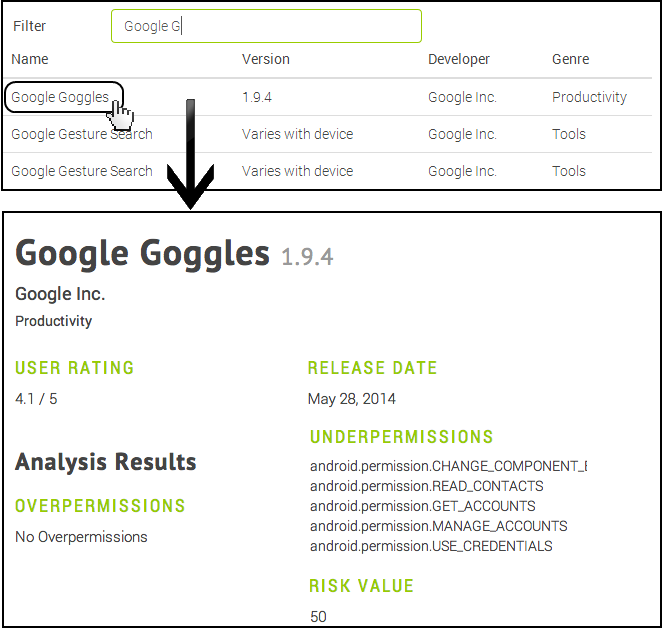
\includegraphics[width=\columnwidth, angle = 0]{images/screenshot3.png}
\caption{\ifisnopii darwin.rit.edu \else xxx.hidden.edu \fi Website Reporting Tool}
\label{fig:website1}
\end{figure}


 \begin{figure}[ht!]
\centering
%\frame{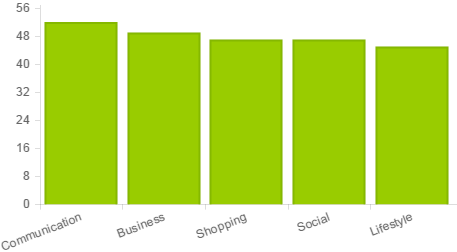
\includegraphics[scale=.5]{images/overprivsByGenre.png}}
%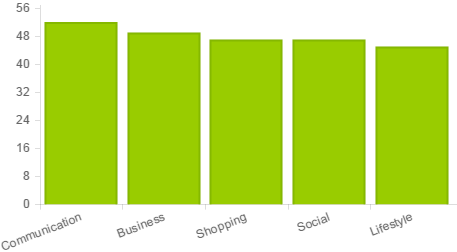
\includegraphics[scale=.7]{images/overprivsByGenre.png}
 \par\framebox[1.1\width]{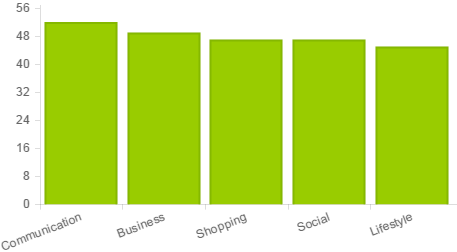
\includegraphics[scale=.63]{images/overprivsByGenre.png}}
\caption{Overprivileged Apps By Genre from Project Website}
\label{fig:overprivappsByGenre}
\end{figure}


%The website also includes several data driven result sets about apps at a more aggregate level. Figure~\ref{fig:overprivappsByGenre} shows an example graph with the percentage of apps in the top 5 genres which contain at least 1 overprivilege.

The website also includes several data driven result sets about apps at a more aggregate level. One example is shown in Figure~\ref{fig:overprivappsByGenre}, which displays an example graph with the percentage of apps in the top 5 genres which contain at least 1 over-permission.




% http://darwin.rit.edu/reports
There are 16 prebuilt reports in .csv format which are available in several areas including the rate at which two over-permissions appear together in all applications, the percentage of times each over-permission occurs in all applications, and the percentage of times each over-permission occurs in all applications.


As shown in Figure~\ref{fig:webpagequery}, users may also explore the data by writing their own queries against the dataset right on the webpage.

\begin{figure}[ht!]
\centering
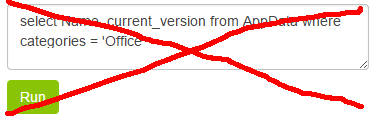
\includegraphics[width=\columnwidth, angle = 0, scale=.8]{images/webpageQuery.png}
\caption{Webpage Search Query}
\label{fig:webpagequery}
\end{figure}




\subsection{Malware Information}
The raw data used in our analysis is available in three SQLite databases from our public GitHub repository, with one each for the malware data from Contagio and the Malware Genome projects, and a third for the collected information from Google Play.

The databases schemas are constructed in a similar format to one another and contain views that make data analysis easier. Further information regarding these views, along with ER diagrams to visually represent the dataset are available on the project website. The website also contains prebuilt reports with data available in a variety of formats including html, pdf, xls, and csv; users are also able to build their own reports. Unfortunately, the actual malicious APK files may only be obtained from the Contagio and Genome websites due to usage agreements.



\section{Limitations \& Future Work}
\label{sec:limitations}


While static analysis tools have demonstrated their value in numerous previous works~\cite{Felt:2011:APD:2046707.2046779, Pearce:2012:APS:2414456.2414498}, it is unreasonable to expect that any tool will ever be flawless and that no static analysis tool is perfect and generally inherently contains limitations~\cite{chess2004static}. Although Stowaway is a powerful static analysis tool which has been used in previous research~\cite{Pearce:2012:APS:2414456.2414498,Stevens_investigatinguser,jeon2011dr}, it does suffer from drawbacks. Stowaway's own authors state that the tool only achieves 85\% code coverage~\cite{Felt:2011:APD:2046707.2046779}, so the under \& over-permissions reported by this tool are imperfect. Additionally, any reported vulnerabilities or defects by a static analysis tool should be deemed as~\emph{possible} vulnerabilities or defects, not necessarily actual ones. There is also the possibility of issues in the reverse engineering process of the apps, but we are confident in the process due to its demonstrated effectiveness and accuracy in existing research~\cite{krutz2015FDroid, Lee_2013}, and due to our manual verification of some of the apps.

Identifying possible vulnerabilities or security risks is extremely difficult, and like any static analysis tool Androrisk is only capable of making educated observations about the risk level of an app and that more substantial risk assessments will require a far more substantial level of analysis, which will likely include a manual investigation of the app. Due to the large number of examined apps in our study, this thorough level of analysis was not practical. Even with almost certain imperfections, we believe that Androrisk was a good choice due to its ability to quickly analyze apps and its use in existing research~\cite{krutz2015FDroid}.

We compiled much of our data through reverse engineering APK files from the Google Play store. While similar reverse engineering techniques have been successfully used in previous works~\cite{Lee_2013,6687155}, no reverse engineering process can ever be expected to be totally accurate. However, based on manually verifying a small subset of our results and previous research, we have a high confidence in our reverse engineering process.


We only analyzed apps from Google Play and not other sources such as AppksAPK or F-Droid, which would have led to more varied application origins. However, we feel the diversity of our apps was already quite robust since we collected 70,785  applications from 41 genres. We also only examined free applications in our research due to cost constrains. Thus, the measurements comparison of apps is not representative of the entire Google Play market. Our results only apply as an evaluation of free apps, not paid apps.

We analyzed 1,420 malicious Android apps in a variety of areas. Although this represents a substantial number of malicious apps, it obviously represents only a minor portion of all Android malware. Attaining Android malware samples is a difficult task since they are often difficult to identify, and are often not widely publicized or shared for a variety of reasons, including the fear that this may only lead to them spreading.

While we have demonstrated profound results through the collection of over 70,000 Android apps, future work may be conducted in several key areas. We only analyzed free apps, and an interesting study would be to compare the free and paid apps using a similar process as ours. Future studies could also analyze how apps evolve over time through the examination of numerous released versions of the same app. Android 6.0 received a massive permissions overhaul and work may be done to see how this new release affects how developers use permissions. Naturally more apps can always be examined, and with new apps being released on a daily basis the process is never ending. Additional research may also be done to examine apps collected from other sources, such as AppksAPK or F-Droid.

We used Stowaway to discover over-permissions in apps. While permission misuse is a possible vulnerability, over-permissions do not necessarily mean permission leaking, which is when an unprivileged app has access to permissions which is was never granted. Often, an app is allowed access to permissions by inheriting permissions from another app with the same signing key~\cite{felt2011permission, grace2012systematic}. Future work using permission leak detection tools such as IntentFuzzer~\cite{Yang:2014:IDC:2590296.2590316} can be done to include this metric in the app's security analysis.





%   ? Adoption rates of new Android APis    - Might not be a great idea to include this
%   Further undestanding of what these values mean
%   Website enhancements


%%  What was said in evaluations that we can address here



\section{Conclusion}
\label{sec: conclusion}

We reverse engineered over 70,000 Android apps from the Google Play store and 1,420 malicious apps and then analyzed them using several quality and security static analysis tools. Some of our primary findings include......


Have also laid the groundwork for future work in a variety of areas


\todo{finish}

%%% Remove this section if there are space issues
\section*{Acknowledgements}

%\ifisnopii http://darwin.rit.edu \else http://xxx.hiddenToKeepAnonymous.edu \fi
\ifisnopii
We would like to thank the following students for their contributions on this project: Casey Klimkowsky, Shannon Trudeau, and Adam Blaine. This research would not have been possible without their hard work, ingenuity and dedication to the project.

\else
Hidden to protect review anonymity
\fi




\balance
\bibliographystyle{abbrv}
\bibliography{SecurityDarwin}



% That's all folks!
\end{document}


%%%% Todo
% Make sure that the format is correct
% Keywords
% Make sure app counts (GP, Malware etc...) all match up
% under-permission, over-permission
% convert to SEFM format



%%% Feedback:
% Make the contribution of the paper very clear
% Actionable results
% Analyze observed relationships






%% Notes
% `dataset` or `data set` -
%   Use the term "overprivilege"
